\section{実関数の計算量}
\label{section: preliminaries}

\subsection{実関数の計算}

実数を文字列から文字列への関数で表す.
 \begin{definition}
  関数$\phi \colon \{0\} ^* \to \{0, 1\}^*$が実数$x \in \R$の\emph{名}であるとは,
任意の$n \in \N$について, 
  $\phi(0^n) = \lfloor x \cdot 2^n \rfloor$ または
  $\phi(0^n) = \lceil x \cdot 2^n \rceil$ を満たすこと.
 \end{definition}
ここで$\lfloor \cdot \rfloor$, $\lceil \cdot \rceil$とはそれぞれ
整数へ切り捨てた値, 及び切り上げた値を二進法で書いた文字列を表す.
つまり実数$x$の名は, 
長さ$n$の文字列$0 ^n$を受け取ると, 精度$n$桁の$x$の
近似値を返す.

この名を読み書きする機構として, 
神託チューリング機械 (以下単に機械という) を使う(図\ref{fig:model-of-function}).
% 計算可能な実関数は Grzegorczyk によって初めて形式的に定義された
% \cite{grzegorczyk1955computable}.

 \begin{figure}
  \begin{center}
   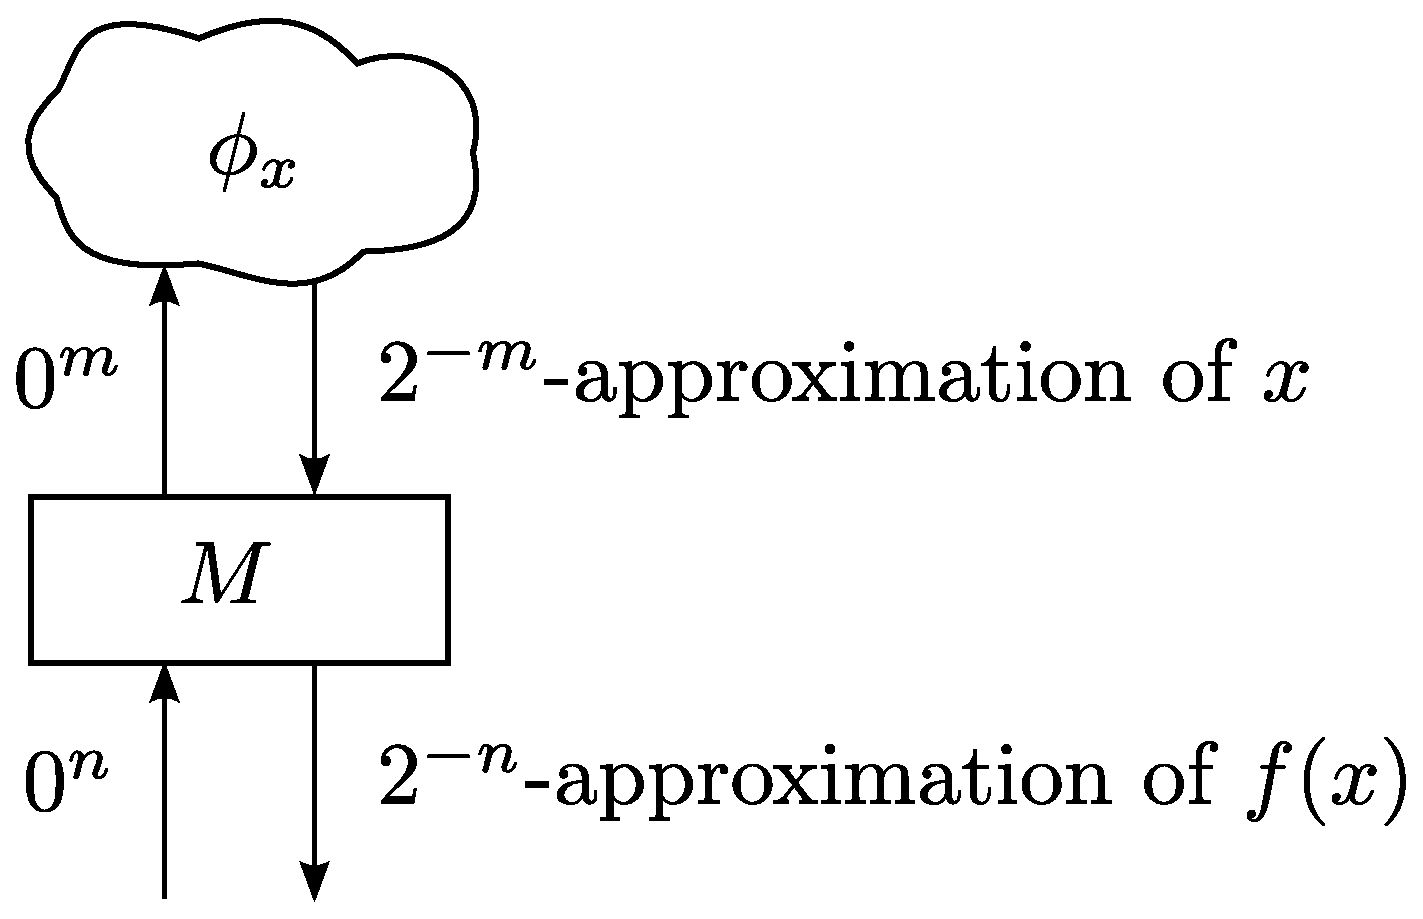
\includegraphics[height=0.15\textheight]{image/model-of-function.eps}
  \end{center}
  \caption{実関数$f$を計算する機械$M$}
  \label{fig:model-of-function}
 \end{figure}

機械$M$に, 
文字列から文字列への関数$\phi$を神託として与え, 
文字列$0 ^n$を入力として与えたとき, 
出力される文字列を$M ^\phi (0 ^n)$で表す. 
つまり$M ^\phi$をやはり文字列から文字列への関数とみる. 

\begin{definition}
$A$を$\R$の有界閉区間とする. 
機械 $M$ が実関数 $f \colon A \to \R$ を計算するとは,
任意の実数 $x \in A$, 任意の $x$ の名 $\phi_x$ に対して,
$M^{\phi_x}$ が $f(x)$ の名であること.
\end{definition}

$A$が$\R ^2$の有界閉集合であるときにも, 
神託を二つ取る機械を考えて同様に定義する. 

 ある実関数が\emph{計算可能}であるとは, その関数を計算する神託機械が存在することである.
 同様に, ある実関数が\emph{多項式時間計算可能}であるとは, その関数を計算する多項式時間神託機械が存在することである.

 神託機械 $M$ で $f$ を計算するとき, 求める$f (x)$の精度 $n$ に対して,
 $x$ の近似値に必要な精度 $m$ が定まるため,
 計算可能な関数は連続である.
 また $n$ と $m$ の対応関係と有理数における近似値を与えることで,
 計算可能実関数や多項式時間計算可能実関数に対して,
 神託機械を用いない同値な特徴付けが可能である.

\begin{lemma}
  \label{lem:type1representation}
  実関数$f\colon [0,1] \to \R$が多項式時間計算可能であることは, 
  多項式時間計算可能な
  関数$\phi \colon (\Q \cap [0, 1]) \times \{0\} ^* \to \Q$と
  多項式$p \colon \N \to \N$とが存在し, 
  任意の $d \in \Q \cap [0,1]$, $n \in \N$ について
  \begin{equation}
   |\phi(d, 0^n) - f(d)| \le 2^{-n} 
  \end{equation}
  任意の $x, y \in [0, 1]$, $m \in \N$ について
  \begin{equation}
   |x-y| \le 2^{-p(m)} \Rightarrow |f(x) - f(y)| \le 2^{-m} 
  \end{equation}
  が成立つことと同値である. 
但し$\Q$の元は分母と分子を二進法の整数で書いた分数として表す. 
\end{lemma}

\subsection{帰着と困難性}

言語$L \subseteq \{0, 1\} ^*$は
関数$L \colon \{0, 1\} ^* \to \{0, 1\}$と同一視し, 
$u \in L$のとき$L (u) = 1$とする. 

\begin{definition}[帰着]
  言語$L$が実関数$f \colon [0, 1] \to \R$に\emph{帰着}するとは, 
  多項式時間計算可能な関数 $S$ と多項式時間神託機械$M$が存在し, 
  任意の文字列 $u$ に対して以下を満たすことをいう(図\ref{fig:reduction}). 
 \begin{figure}
  \begin{center}
  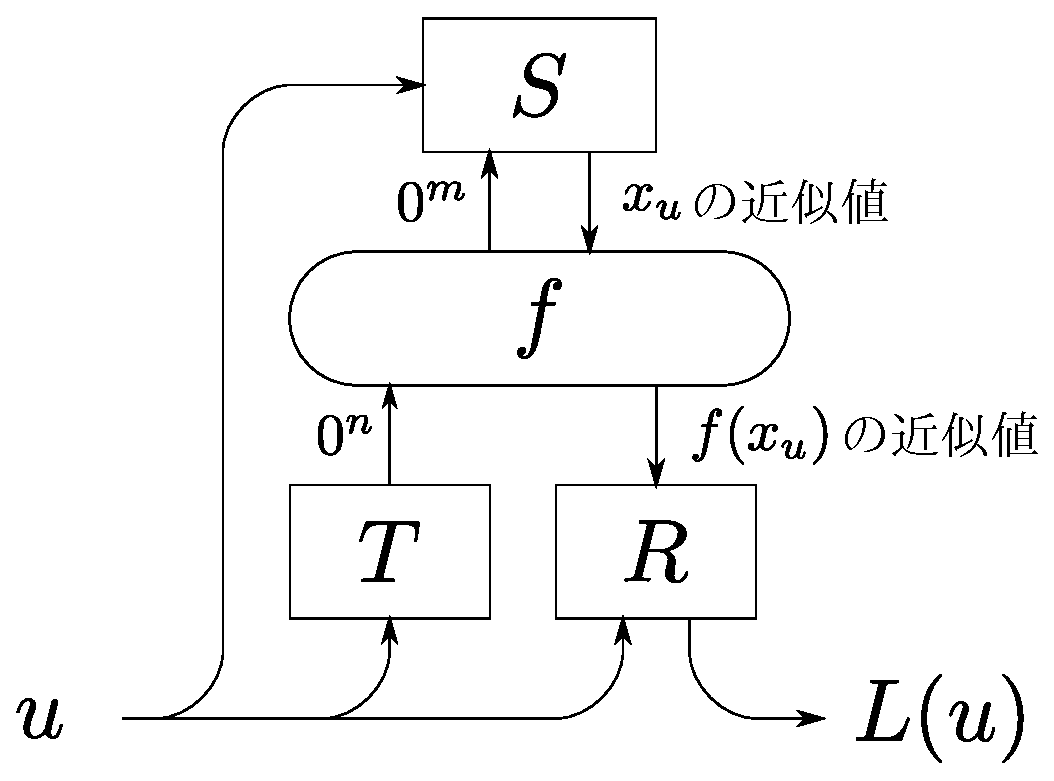
\includegraphics[scale=0.25]{image/reduction.eps}
  \caption{言語$L$から関数$f \colon [0,1] \to \R$への帰着}
  \label{fig:reduction}
  \end{center}
 \end{figure}
  \begin{itemize}
   \item $S(u, \cdot)$ はある実数 $x_u$ の名;
   \item $f(x_u)$ の任意の名 $\phi$ に対して
	 \[
	  M^\phi(u) \text{が受理} \leftrightarrow u \in L.
	 \]
  \end{itemize}
\end{definition}
 この定義は河村による帰着の定義と形式上は異なるが,
 帰着としての強さは等しい.
 計算量 $C$ に対して, 関数 $f$ が \emph{$C$ 困難}であるとは,
 $C$ に属する任意の言語が $f$ に帰着することをいう.
